\chapter{Diskussion}
I denne sektion vil resultater, fremført i afsnit \ref{sec:resultater}, fortolkes og kommenteres, for at besvare de opstillede problemstillinger. \\ \\
Først og fremmest var det interessant for dette projekt, at udlede hvorvidt det var muligt at opnå en korrekt korrespondanceanalyse af markbillederne, dvs. at udvælge korrekte korresponderende punkter. Opgavens hovedproblemstilling omhandler bestemmelsen af, hvilke af de udvalgte metoder, der bedst muliggør en korrekt korrespondanceanalyse af markbillederne. For at kunne konkludere ovenstående, iagttages to aspekter fra resultaterne: (1) Hvor mange korrekte korrespondancer, hver metode har fundet. (2) Hvor mange korrekte korrespondancer, hver metode har fundet, ift. mængden af de detekterede interessepunkter. Disse to aspekter er opstillet i nedenstående tabel og opsummere opgavens resultater.
\begin{center}
    \begin{tabular}{ | l | l | l | l |}
    \hline
    Detektor & Deskriptor & $\text{Match(A,A')}$ & $\text{mean rm}$ \\ \hline
    $DoH$ & SURF & 1846.8 & 0.15063 \\ \hline  
    Harris & SIFT & 318.7 & 0.1505 \\ \hline    
    Moravec & SIFT & 293.3 & 0.13926 \\ \hline    
    $DoG$ & SIFT & 268.2 & 0.02916 \\ \hline         
    \end{tabular}
    \label{table:tab}
\end{center}
Tabellen viser at det var muligt for alle metoder at udvælge korrekte korrespondancer i billederne, og derved opnå en korrekt korrespondanceanalyse af markbillederne. For at besvare hovedproblemstillingen, evalueres metoderne ud fra deres repeatability measure $rm$. Det kan ud fra dette ses at metode kombinationen $DoG$ \& SURF, bedst muliggør en korrespondanceanalyse af markbillederne. Figur \ref{fig:graf} viser hver metodes repeatability measure, pr. billede.
\begin{figure}[H]
    \centering
    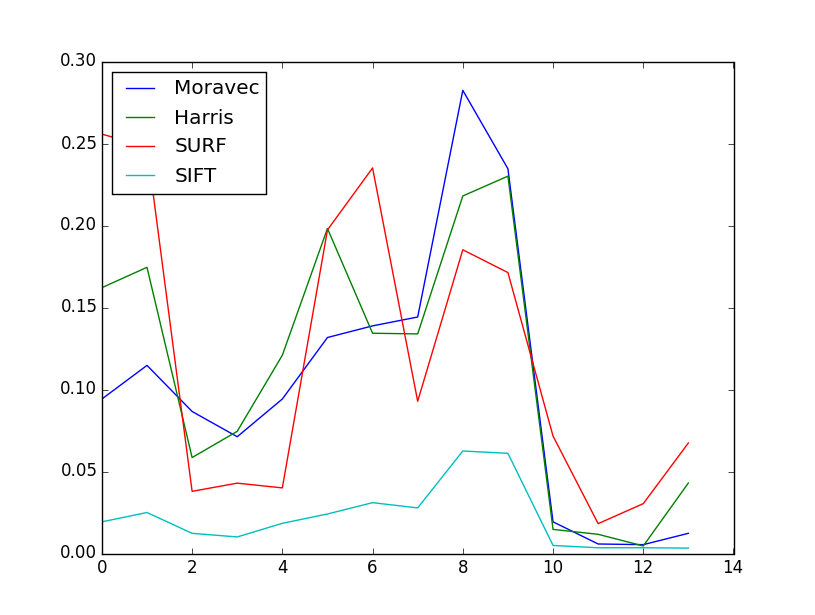
\includegraphics[width=0.65\textwidth]{fig/repeatabilitygraph.png}
     \vspace{-1em}
    \begin{center}        
     \caption{{\footnotesize \textit{
De implementerede metoders repeatability measure, over de forskellige )}}}
    \label{fig:graf}
     \end{center}
       \vspace{-2.5em}
  \end{figure}
\noindent
Det ses at den samlede metode SIFT, gav de dårligste resultater. Dette var overraskende, da SIFT er en metode der i høj grad er anerkendt og bredt anvendt. Denne opgaves implementering af SIFT er diskuteret i afsnit <forbedringer>. Resultaterne for hjørnedetektorene: Harris og Moravec, var overraskende gode og derfor kan det udledes at både hjørne - og blobdetektorer kan anvendes til korrespondanceanalyse af markbilleder.
\\ \\
For metoderne viste det sig at størstedelen af de brugbare punkter, i et stort omfang, blev udvalgt på én specifik oktav. Derfor viser resultaterne kun metoderne anvendt på den oktav, der gav de bedste resultater. Denne beslutning er yderligere beggrundet ved at dronen tager billederne fra én bestemt højde, der forekommer altså ikke højdeændringer i mellem de afprøvede billeder. Derfor kan det konkluderes at selvom størstedelen af de brugbare punkter blev udvalgt på samme oktav, var der behov for en skalarums repræsentation af markbillederne, for at kunne udvælge hvilken oktav, der gav de bedste resultater.
\\ \\
Som set i figur \ref{fig:rota} (øverst) er den ikke-rotationsinvariante deskriptor U-SURF, kun i stand til at etablere meget få korrekte korrespondancer, når billederne er roteret ift. hinanden. (Nederst) ses det at den rotationsinvariante deskriptor SURF er i stand til at udvælge alle korresponderende punkter korrekt. For de to billeder er det derfor nødvendigt at anvende en rotationsinvariant deskriptor, for at opnå en korrekt korrespondanceanalyse. De to udvalgte billeder repræsentere dog ikke resten af billedsættet, da der ikke forekommer en så markant rotation imellem de andre billeder. Derfor er det kun et isoleret tilfælde at deskriptoren skal være rotationsinvariant. Denne påstand er yderligere beggrundet ved at det også har været muligt at etablere et stort antal korrekte korrespondancer ved brug af U-
SURF.
\begin{figure}[H]
    \centering
    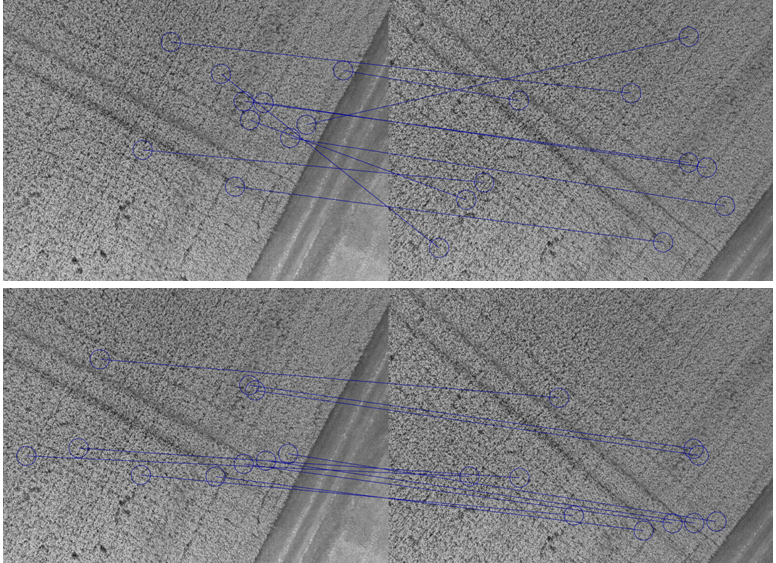
\includegraphics[width=1\textwidth]{fig/rot2.png}
     \vspace{-1em}
    \begin{center} 
       \caption{{\footnotesize \textit{Øverst: De 10 bedste matches fra $DoH$, U-SURF er illustreret. Nederst: De 10 bedste matches fra $DoH$ SURF er illustreret. }}}
    \label{fig:rota}
     \end{center}
     \vspace{-2.5em}
  \end{figure} \noindent
\section{Forbedringer}
Følgende afsnit vil gennemgå hvilke forbedringer de implementerede metoder kan gennemgå, for at forbedre korrespondanceanalysen.
\subsection{Non-maximal suppression}
Som beskrevet i afsnit \ref{sec:dog}, og som gør sig gældende for både Difference of Gaussian og Determinant of Hessian metoderne,  er non-maximal suppression ikke implementeret for at finde sub-pixel nøjagtighed. 
\\
\\
I denne implementering bliver et punkt kun valgt, hvis $|\hat{x}| < 0.5$, i en given retning. $\hat{x}$ angiver en retningsvektor i tre dimensioner$(x, y, \sigma)$, der er orienteret mod et ekstrema og bruges i denne implementering til at frasortere punkter, der ikke er placeret på ekstremaer. Punkters placering er ikke blevet fundet ned til sub-pixel nøjagtighed. Det blev ikke anset som en nødvendighed i denne udgave, da første prioritet var at finde korrespondancer og illustrere dem - her er sub-pixel nøjagtighed ikke brugbart, da hver billedkoordinat er et naturligt heltal. I en praktisk anvendelse, kan det ønskes, at der skal etableres homografier, eller bruge andre billedanalytiske metoder, på de fundne korrespondancer. Her er sub-pixel nøjagtighed strengt nødvendigt, for at få nøjagtige resultater. Implementering af non-maximal suppression som forklaret af Lowe, er derfor næste logiske udvidelse af programmet. 

\subsection{SIFT}
I figur \ref{fig:graf}, ses det, at den udregnede repeatability measure for SIFT er langt lavere, end de andre metoder. Det er lykkedes at finde korrespondancer med den samlede SIFT metode, der er dog langt færre matches, end i Harris/SIFT og SURF. Dette resultat er i uoverensstemmelse med andre sammenligninger af metoder\cite{kim} \cite{kim2}. I \cite{kim} sammenligner Pedersen et al. forskellige metoder med billeder udsat for forskellige ændringer, under kontrollerede forhold. En recall rate, der svarer til den repetability measure brugt her til at evaluere metoderne. Pedersen et al. opsætter nogle strengere krav(mere specifikt, tre krav) for, hvornår to punkter korrespondere ($C(I_1, I_2)$), end der gøres i denne opgave. Kim et al. konkludere at Harris og Difference of Gaussian giver bedere resultater end Determinant of Hessian metoden. Denne konklusion er i modstrid med resultaterne præsenteret her. Selvom applikationsområderne er forskellige, forventedes der alligevel en vis lighed imellem resultaterne. Det må derfor, på baggrund af den udledte repeatability measure for SIFT, konkluderes at der er fejl i implementeringen af SIFT.
\subsection{RGB til gråtone}
Som nævnt i afsnit 3.1, blev der anvendt en specifik metode, til at transformere intensiteter i RGB til gråtone værdier. Det kunne være interessant at undersøge, hvorvidt Excess Green(ExG) kan bruges til at øge repeatability measure. ExG kan bruges til at adskille planter fra jord\cite{exg}. Dette kunne skabe større kontrast i billedet og derfor muligvis tydeliggøre blobs og hjørner.
\chapter{Konklusion}
Dette projekt blev tilgået, med ingen foregående viden/ide om hvorvidt det var muligt at opnå en korrekt korrespondanceanalyse. Der er nu afprøvet en række forskellige metoder, der alle bidrager til den samme konklusionen: At det i høj grad er muligt at opnå en korrekt korrespondanceanalyse, af markbilleder. Udover dette har undersøgelsen vist at ud af de afprøvede metoder, muliggør SURF den mest korrekte korrespondanceanalyse af markbilleder. 
Derudover konkluderes det, ud fra resultaterne, at metoderne skal være skalainvariante, men ikke rotationsinvariante, medmindre der forekommer større rotation imellem billederne, som i det isolerede tilfælde illustreret i figur \ref{fig:rota}.  \\ \\
Opgaven udleder hvilke metoder, der bedst kan anvendes til etableringen af ukrudtskortet, i projektet "Droner til monitering af flerårigt ukrudt i korn". Til projektet ønskes en metode, der kan etablere flere korrekte korrespondancer, konsekvent i alle billeder. I dette projekt er et subset af en markoverflyvning udvalgt og for alle disse billeder var det muligt at etablere en stor mængde korrekte korrespondancer. Resultatet af denne opgave kan derfor bruges som en vejledning, for videreudvikling af projektet i praksis. 